\chapter{Reconstruction Results}

\section{Classification}

We apply the best architectures (as found via the hyperparameter scans in the previous section) separately to our electron vs. charged pion and photon vs. neutral pion reconstruction problems.

Figure~\ref{fig:architectures_ROC_comparisons} shows ROC curve comparisons for the two classification tasks. As expected, the electron vs. charged pion classification problem was found to be a simple task, resulting in an area under the curve (AUC) close to $100\%$. For a baseline comparison, the curve obtained for a BDT is also shown. This BDT was optimized using the {\it scikit-optimize} package~\cite{skopt}, and was trained using high-level features computed from the raw 3D arrays. It represents the performance of current (non-deep-learning) ML approaches on these problems.

\begin{figure}[htbp]
\centering
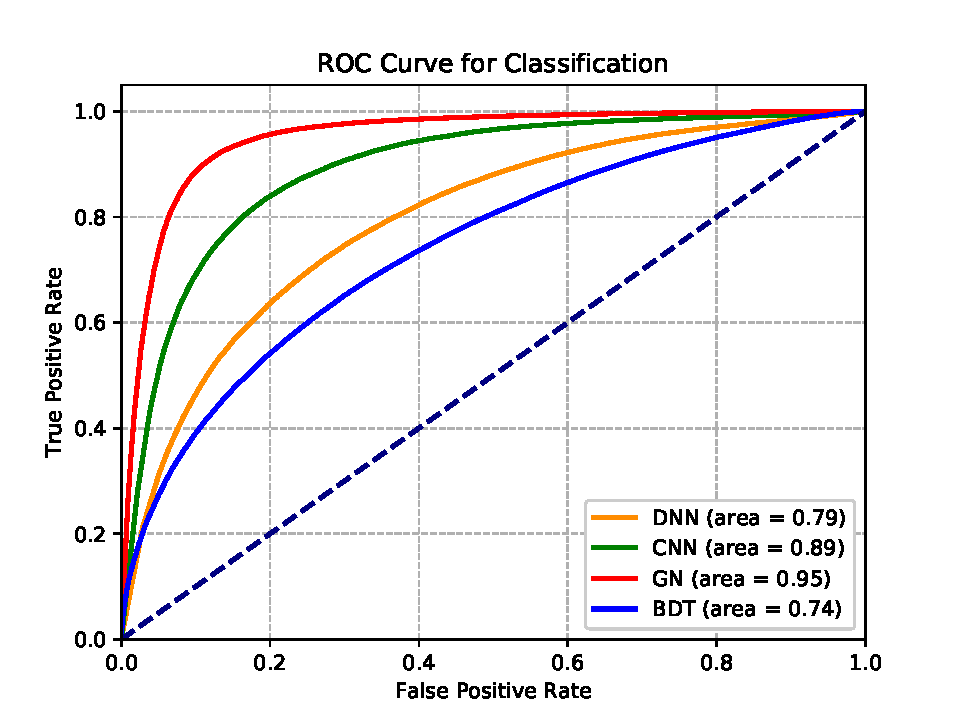
\includegraphics[width=0.45\textwidth]{Images/Calo/architectures_ROC_comparison_gamma_pi0_long.pdf}
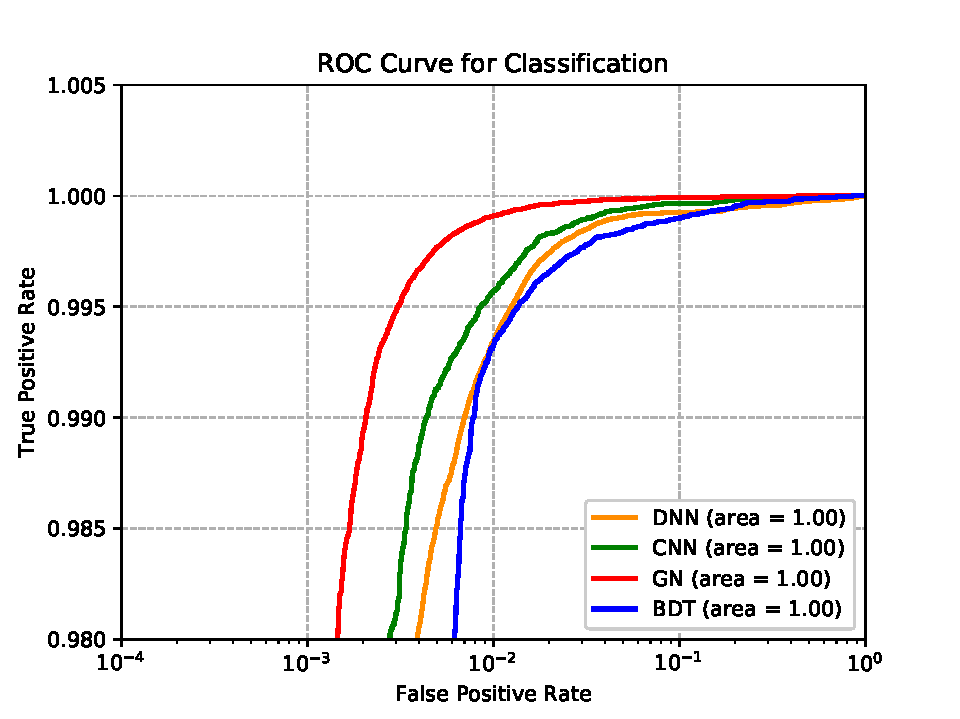
\includegraphics[width=0.45\textwidth]{Images/Calo/architectures_ROC_comparison_ele_chpi_xlog.pdf}
\caption{ROC curve comparisons for $\gamma$ vs. $\pi^0$ (left) and $e$ vs. $\pi^\pm$ (right) classification using DNN, CNN, BDT, and GoogLeNet (GN). Samples include particle energies from 2 to 500 GeV, and an inclusive $\eta$ range.}
\label{fig:architectures_ROC_comparisons}
\end{figure}

Our deep learning models outperform the BDT, with the GN architecture performing best on both problems. Figure~\ref{fig:accuracy_bins} shows the best-model performance as a function of the energy and $\eta$ of the incoming particle, for both classification problems. These figures show that classification accuracy is maintained over a wide range of particle energies and angles. The models appear to perform a bit worse at higher energies for the photon vs. neutral pion case, due to the fact that the pion to two photon decay becomes increasingly collimated at higher energies. Similarly, the performance is slightly worse when particles impact the detector perpendicularly than when they enter at a wide angle, because the shower cross section on the calorimeter inner surface is reduced at $90^{\mathrm o}$, making it harder to distinguish shower features.

\begin{figure*}[htbp]
\centering
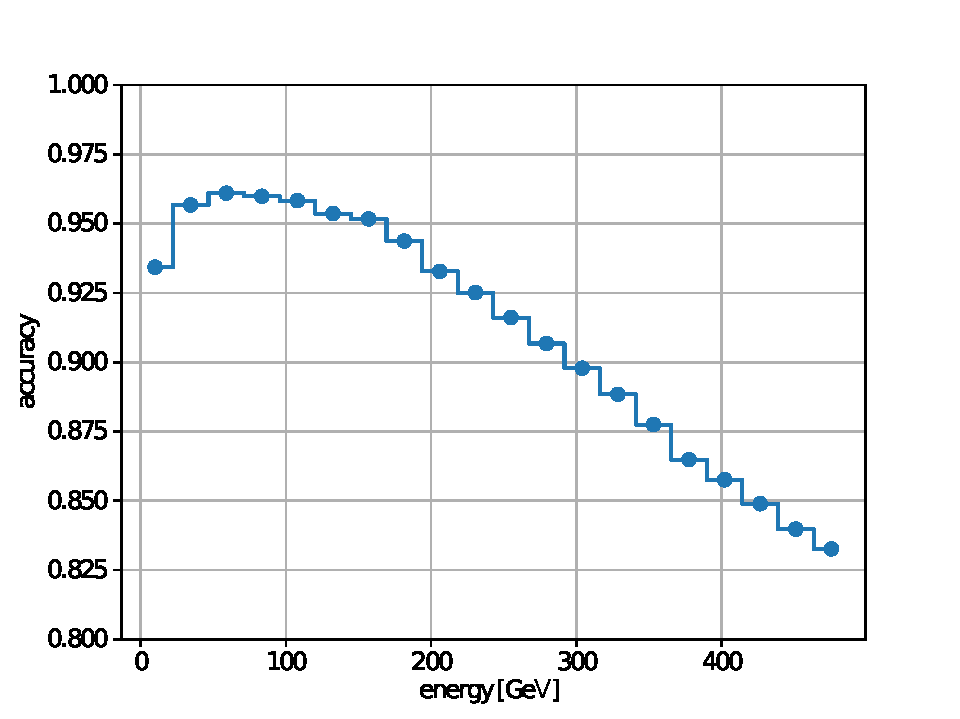
\includegraphics[width=0.45\textwidth]{Images/Calo/gamma_pi0_accuracy_energy_bins.pdf}
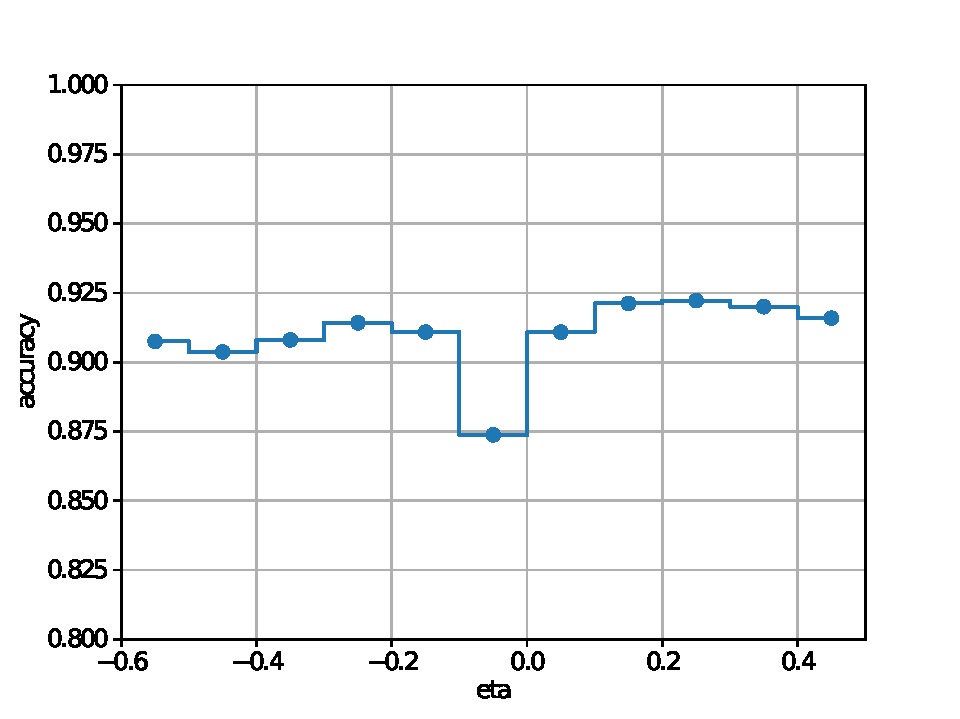
\includegraphics[width=0.45\textwidth]{Images/Calo/gamma_pi0_accuracy_eta_bins.pdf} \\
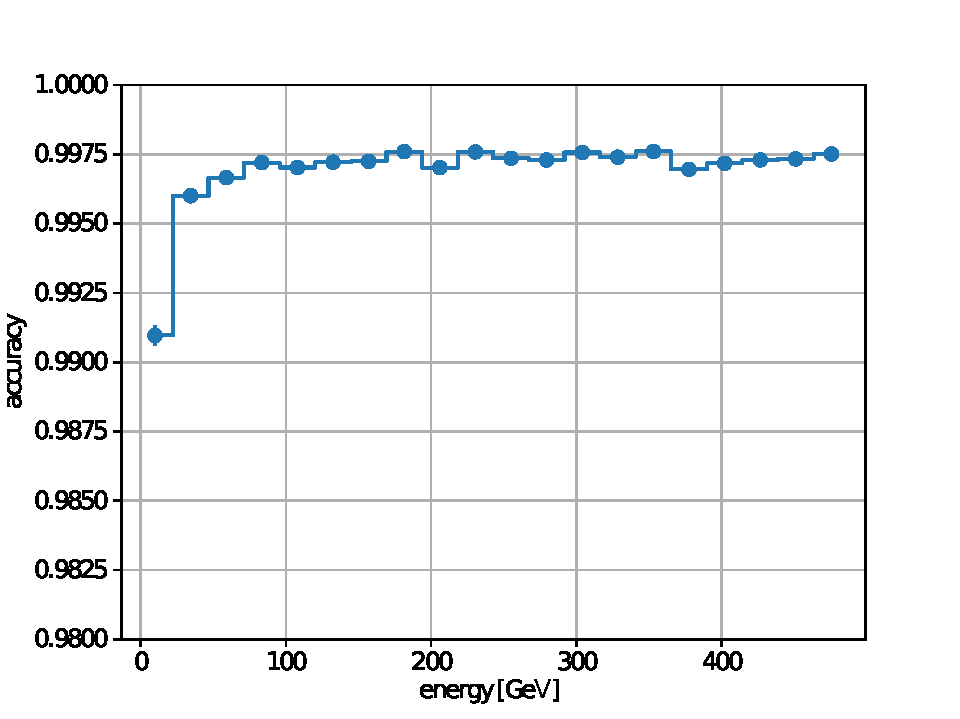
\includegraphics[width=0.45\textwidth]{Images/Calo/ele_chpi_accuracy_energy_bins.pdf}
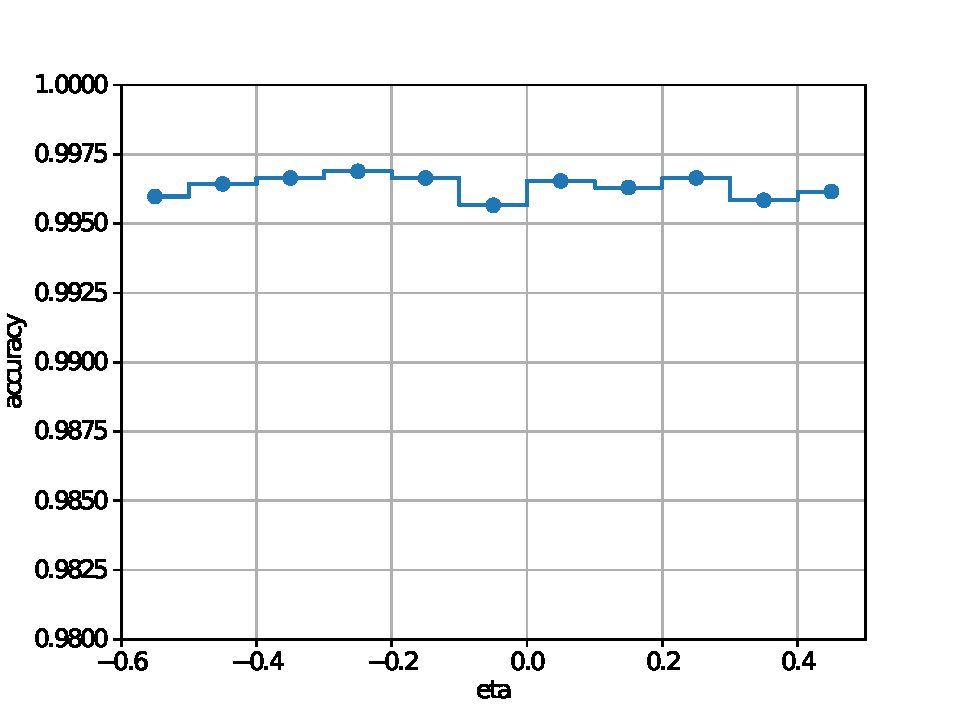
\includegraphics[width=0.45\textwidth]{Images/Calo/ele_chpi_accuracy_eta_bins.pdf}
\caption{Classification accuracy of best performing network for $\gamma$ vs. $\pi^0$ (top) and $e$ vs. $\pi^\pm$ (bottom), in bins of energy (left) and $\eta$ (right).}
\label{fig:accuracy_bins}
\end{figure*}

\section{Regression}

Figure~\ref{fig:reg_dnn_vs_cnn_variable} shows the energy regression performance for each particle type, using each hyperparameter-optimized architecture. We compare against a linear regression and a BDT (labelled as "XGBoost") baseline, as described previously.

\begin{figure*}[htbp]
\centering
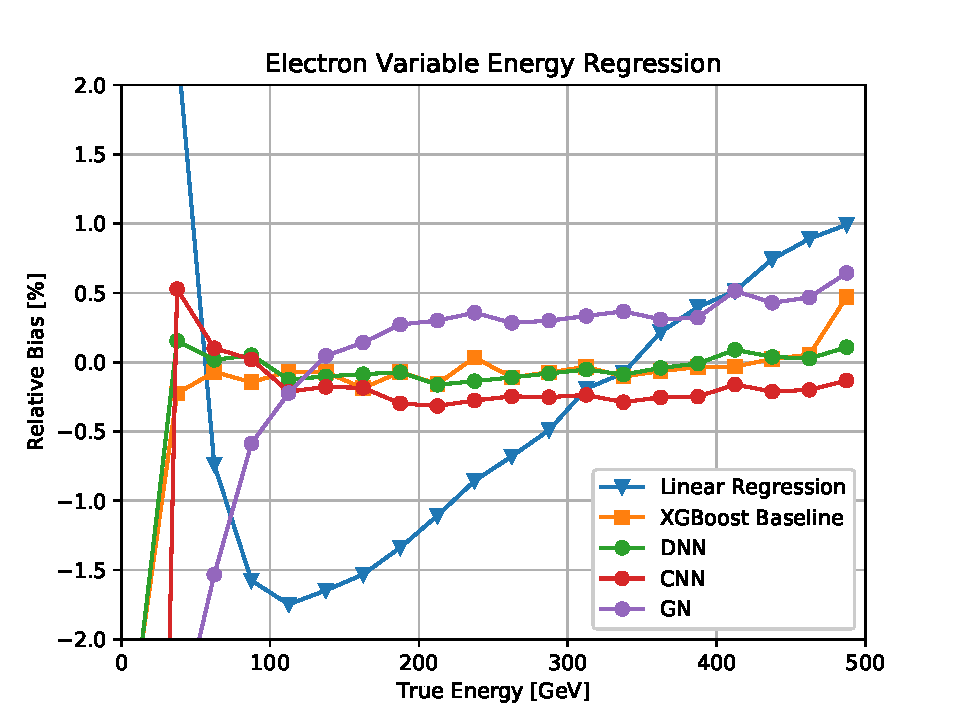
\includegraphics[width=0.45\textwidth]{Images/Calo/bias_vs_E_Ele_variable.pdf}
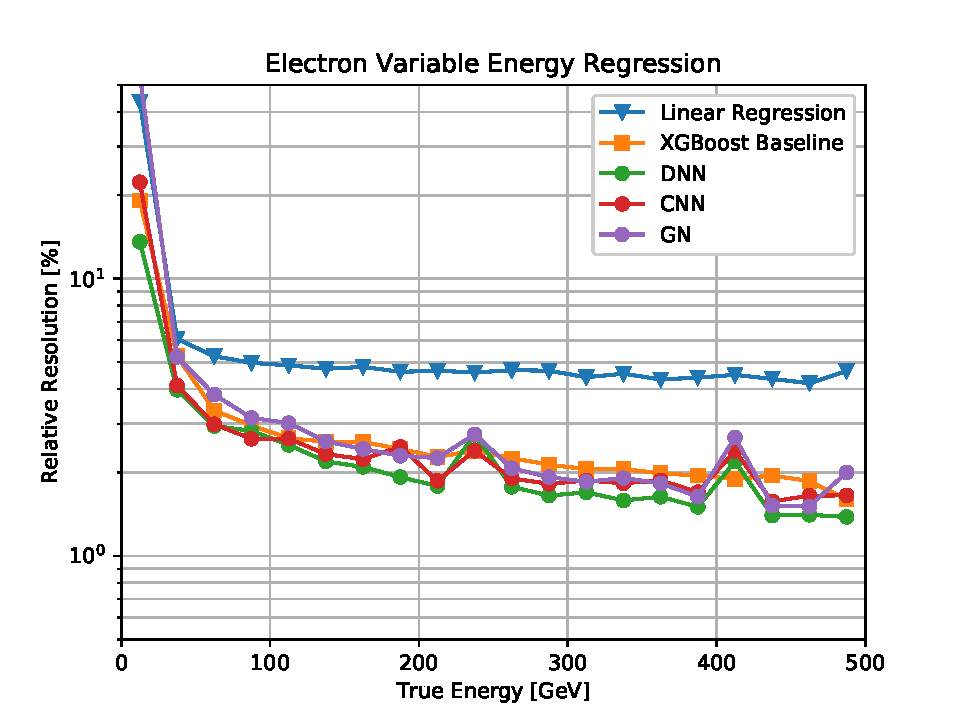
\includegraphics[width=0.45\textwidth]{Images/Calo/res_vs_E_Ele_variable.pdf} \\
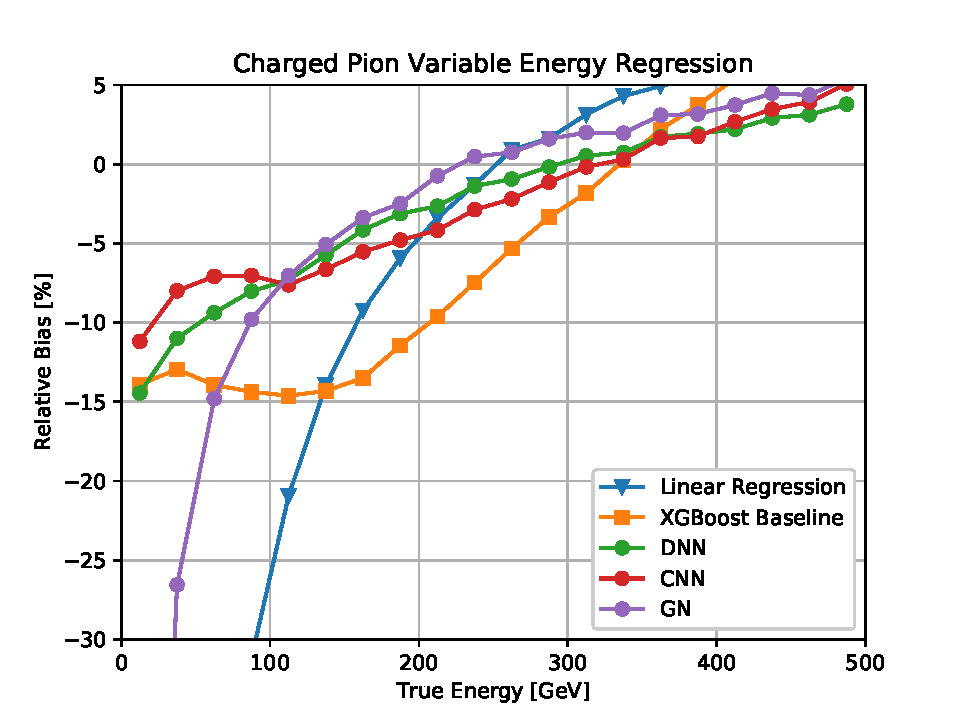
\includegraphics[width=0.45\textwidth]{Images/Calo/bias_vs_E_ChPi_variable.pdf}
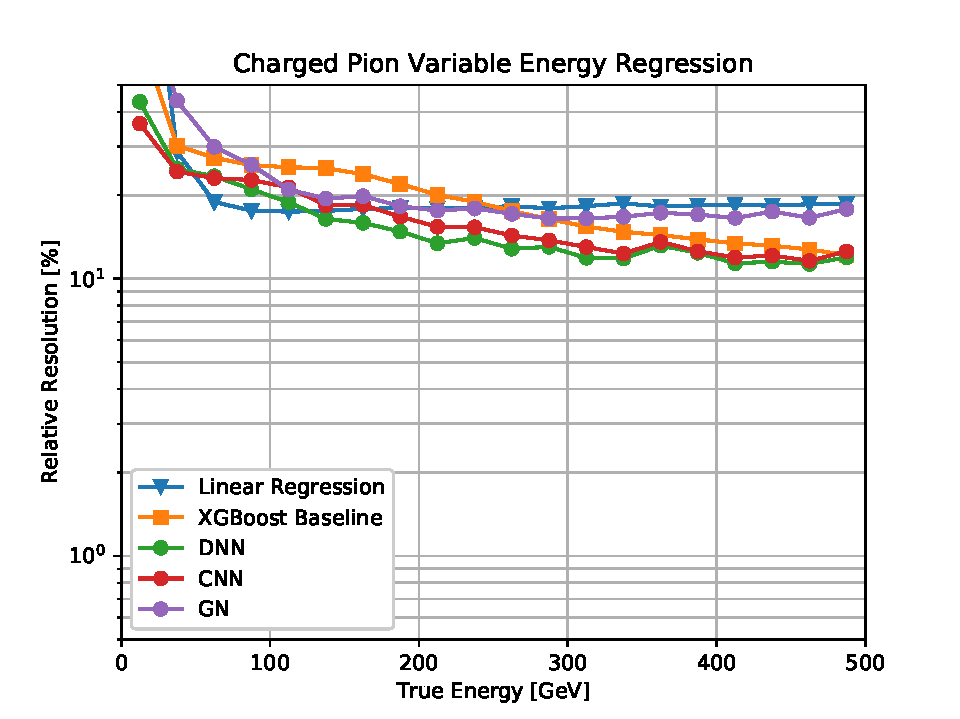
\includegraphics[width=0.45\textwidth]{Images/Calo/res_vs_E_ChPi_variable.pdf} \\
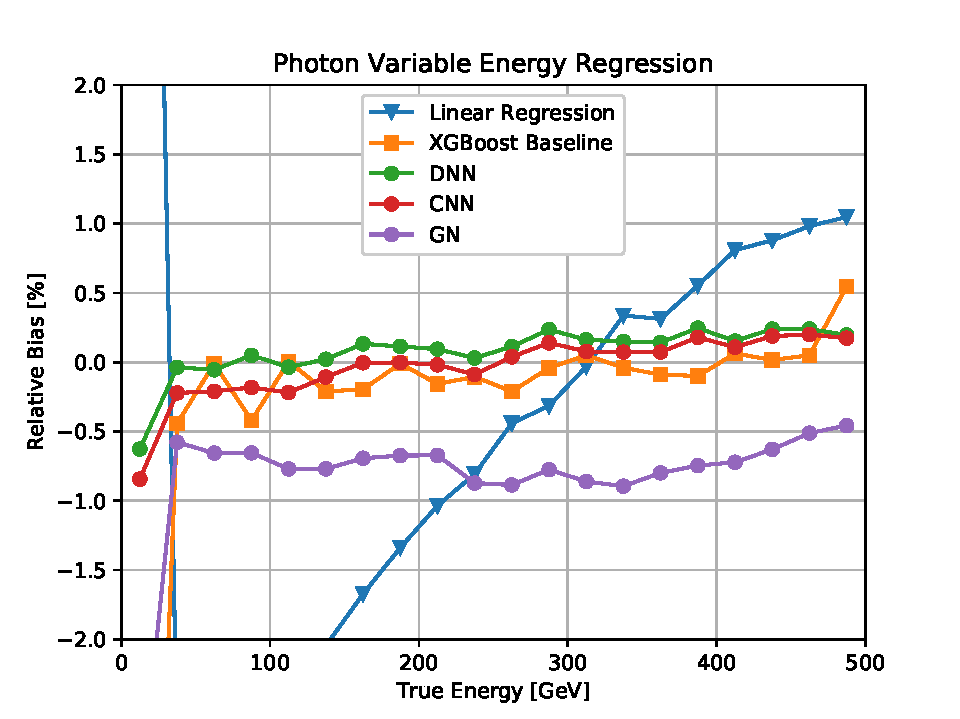
\includegraphics[width=0.45\textwidth]{Images/Calo/bias_vs_E_Gamma_variable.pdf}
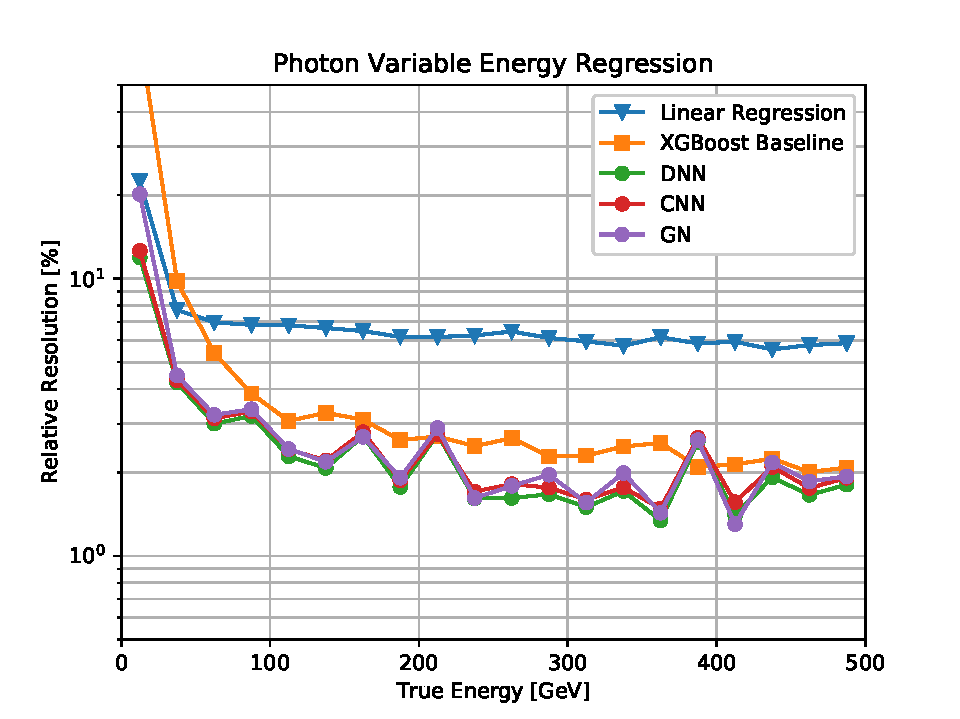
\includegraphics[width=0.45\textwidth]{Images/Calo/res_vs_E_Gamma_variable.pdf}\\
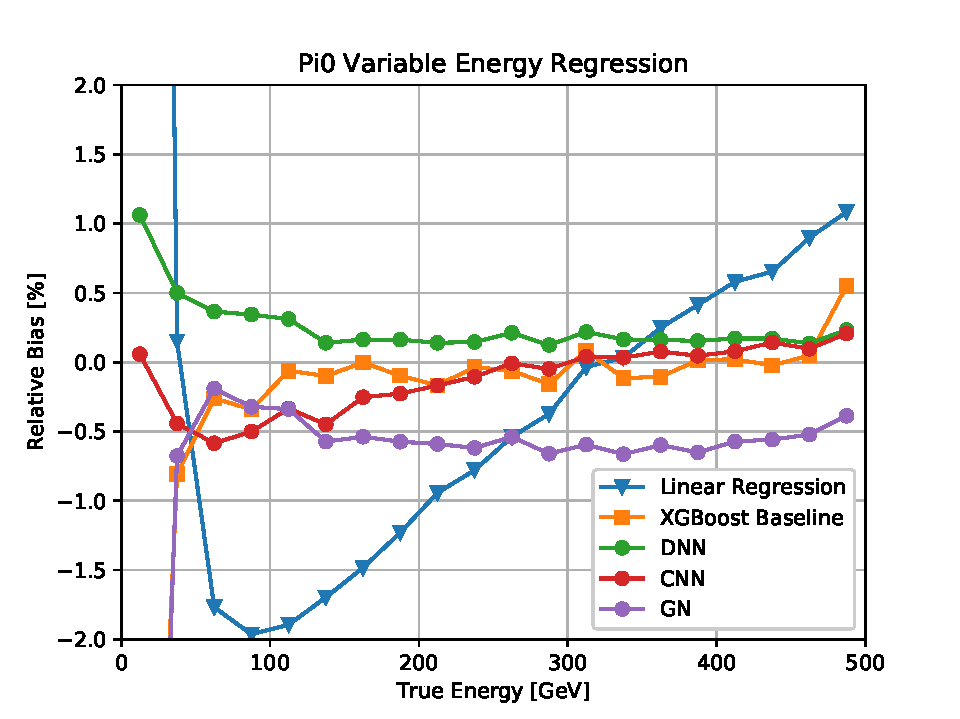
\includegraphics[width=0.45\textwidth]{Images/Calo/bias_vs_E_Pi0_variable.pdf}
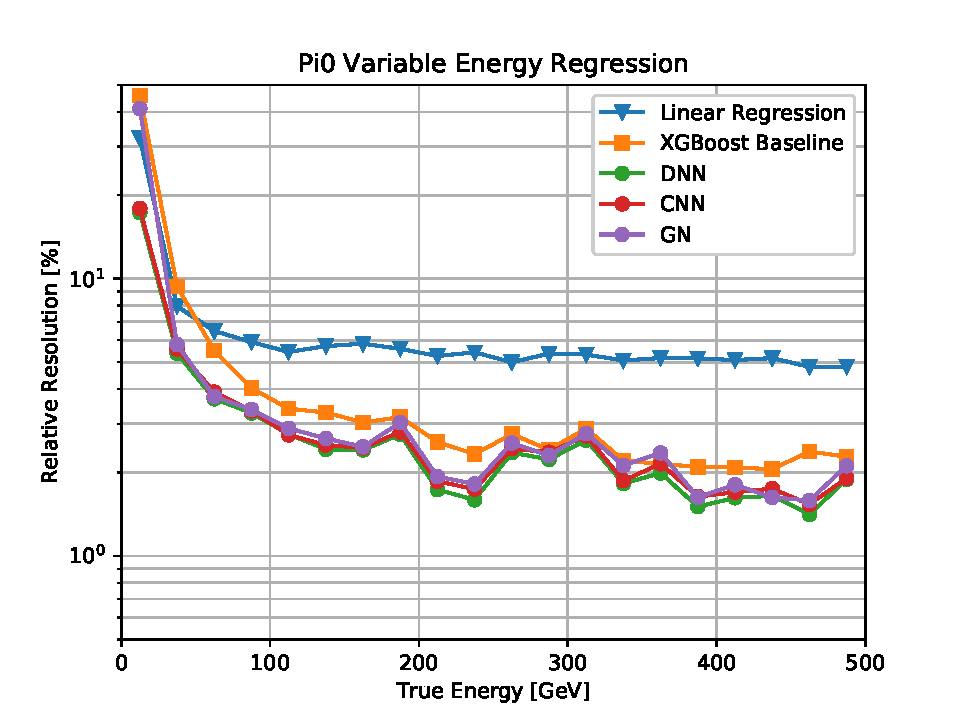
\includegraphics[width=0.45\textwidth]{Images/Calo/res_vs_E_Pi0_variable.pdf}
\caption{Regression bias (left) and resolution (right) as a function of true energy for energy predictions on the REC dataset with variable-angle incident angle. From top to bottom: electrons, charged pions, photons, and neutral pions. Algorithms compared are linear regression, XGBoost (BDT), DNN, CNN, and GoogLeNet (GN).\label{fig:reg_dnn_vs_cnn_variable}}
\end{figure*}

Since the energy regression problem is not as complex as the classification problem, the three architectures (DNN, CNN, GN) perform fairly similarly, with the exception of the GN performance on \chpi, which is a bit worse. The performance is overall worse for \chpi, both with the networks and with the benchmark baselines (linear regression and XGBoost).

A closer look at the performance boost given by each network can be obtained examining the case of particles entering the calorimeter inner surface at $90^{\mathrm o}$, i.e. with $\eta=0$~\footnote{For these additional fixed-angle regression plots, we did not train GoogLeNet architectures.}. In this case, the problem is more constrained and both the networks and the baseline algorithms are able to perform accurately. The results for fixed angle samples are shown in Figure~\ref{fig:reg_dnn_vs_cnn_fixed}.

\begin{figure*}[htbp]
\centering
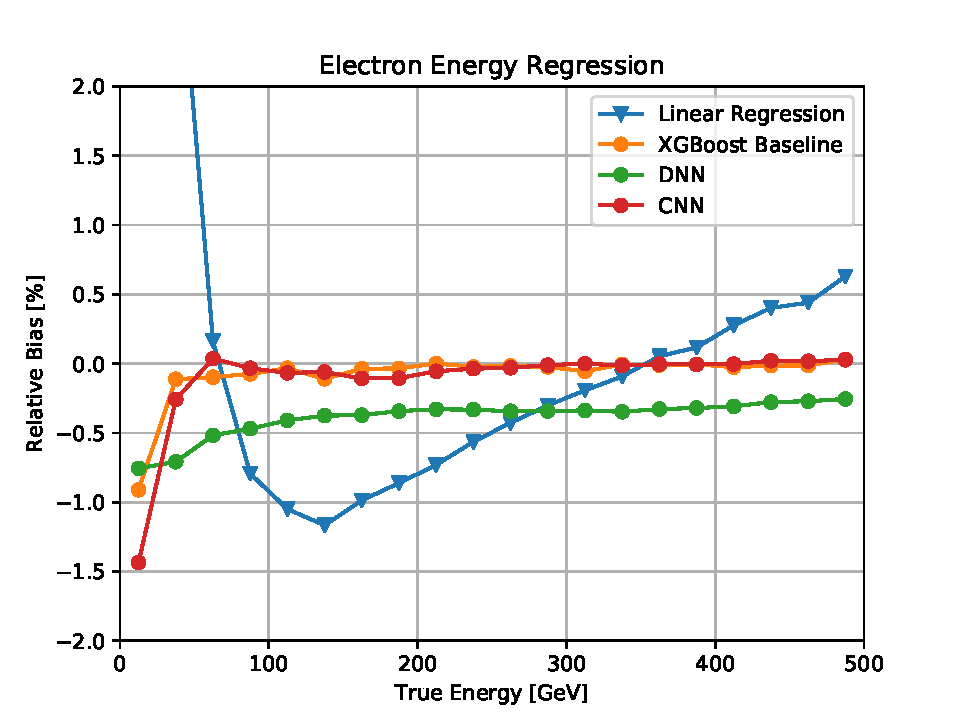
\includegraphics[width=0.45\textwidth]{Images/Calo/bias_vs_E_EleFixed_nn_vs_cnn_zoom.pdf}
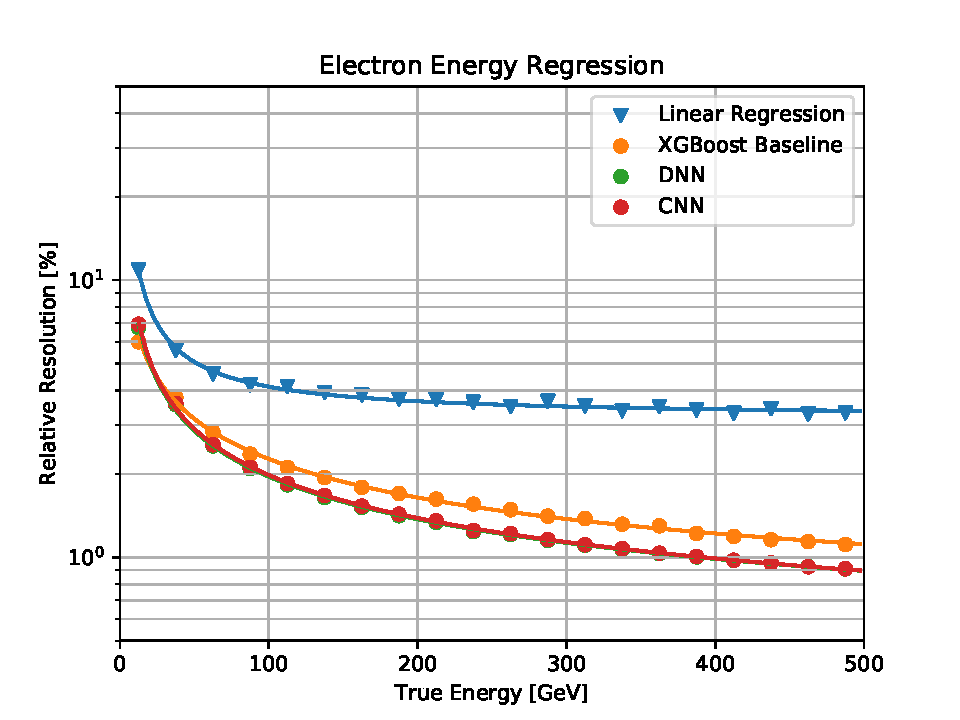
\includegraphics[width=0.45\textwidth]{Images/Calo/res_vs_E_EleFixed_nn_vs_cnn_fits.pdf} \\
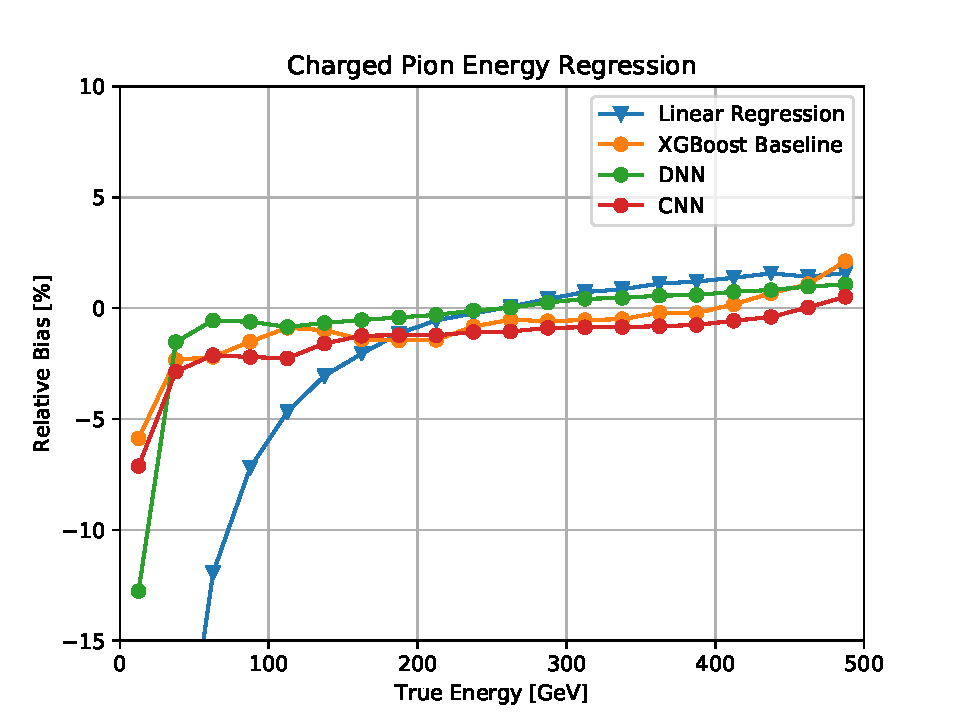
\includegraphics[width=0.45\textwidth]{Images/Calo/bias_vs_E_ChPiFixed_Cut30_nn_vs_cnn.pdf}
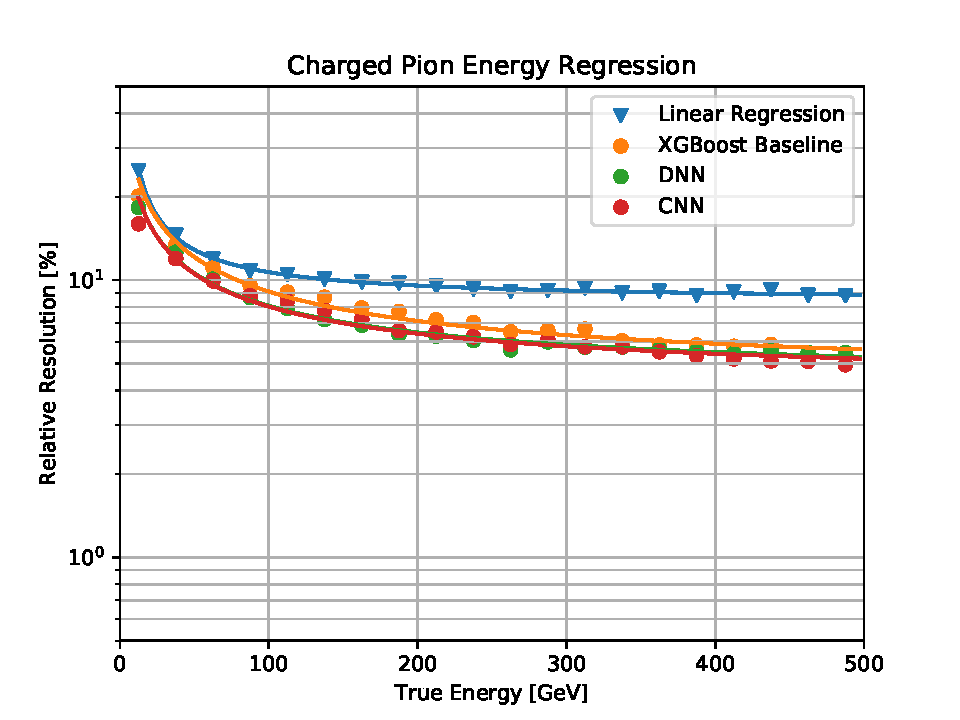
\includegraphics[width=0.45\textwidth]{Images/Calo/res_vs_E_ChPiFixed_Cut30_nn_vs_cnn_fits.pdf} \\
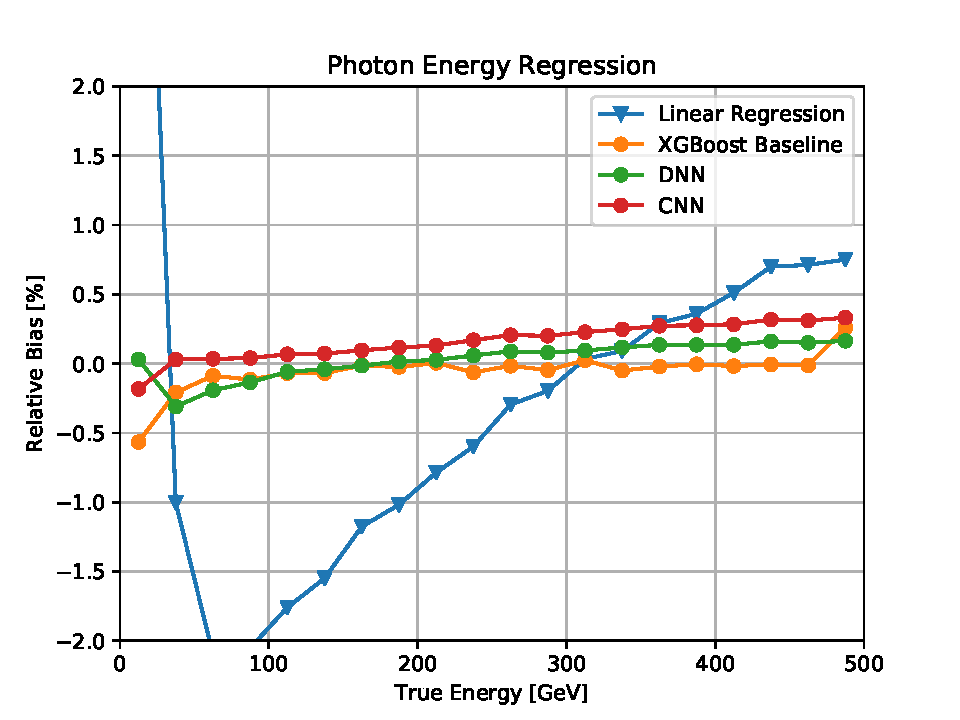
\includegraphics[width=0.45\textwidth]{Images/Calo/bias_vs_E_GammaFixed_nn_vs_cnn_zoom.pdf}
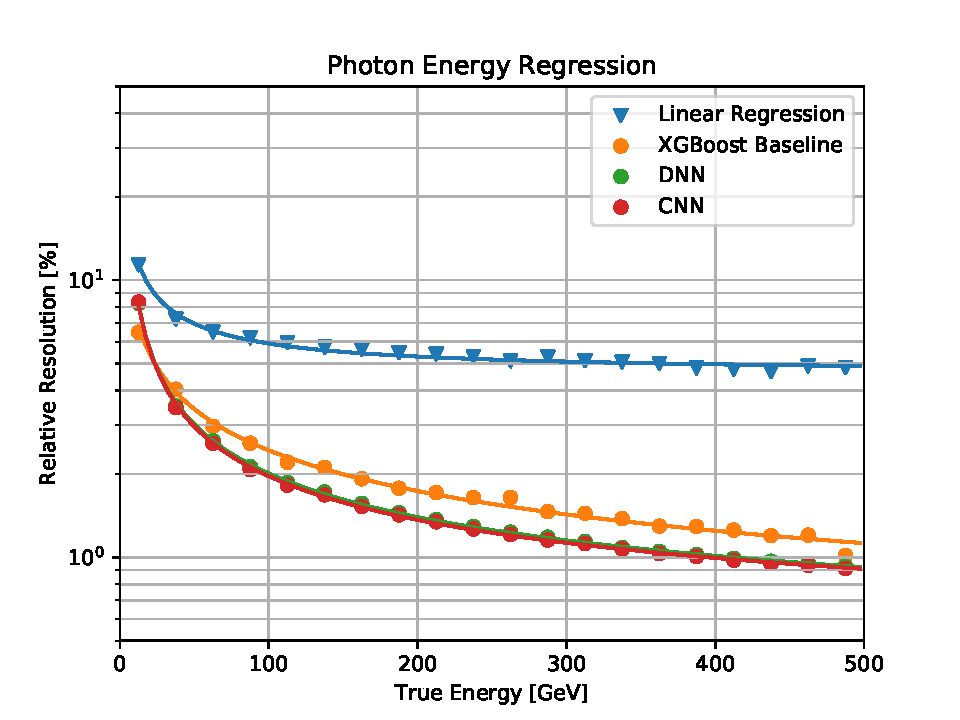
\includegraphics[width=0.45\textwidth]{Images/Calo/res_vs_E_GammaFixed_nn_vs_cnn_fits.pdf} \\
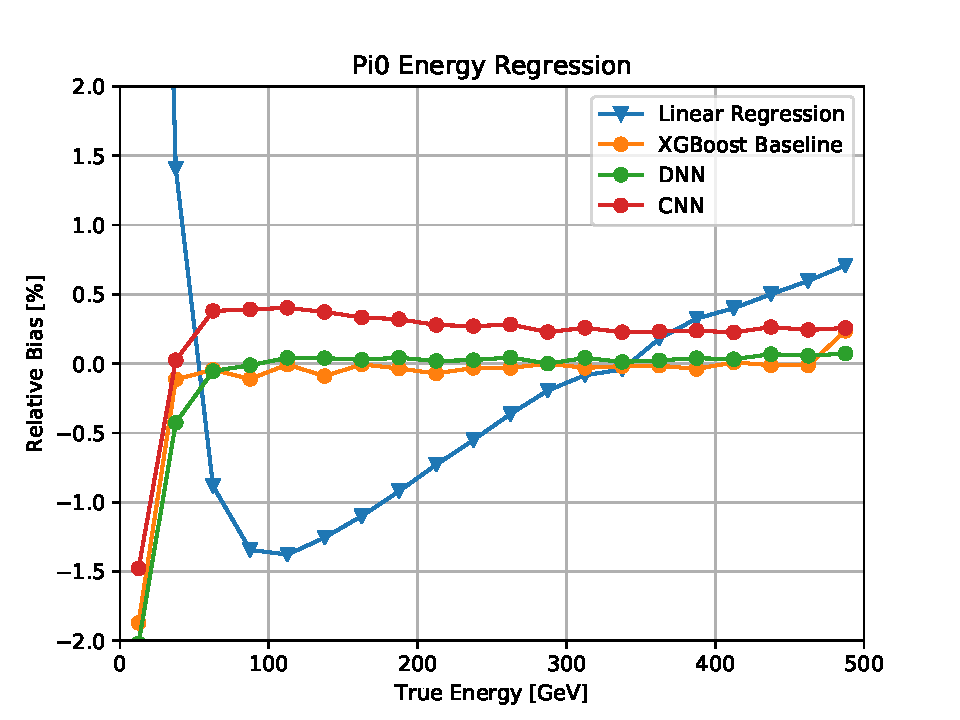
\includegraphics[width=0.45\textwidth]{Images/Calo/bias_vs_E_Pi0Fixed_nn_vs_cnn_zoom.pdf}
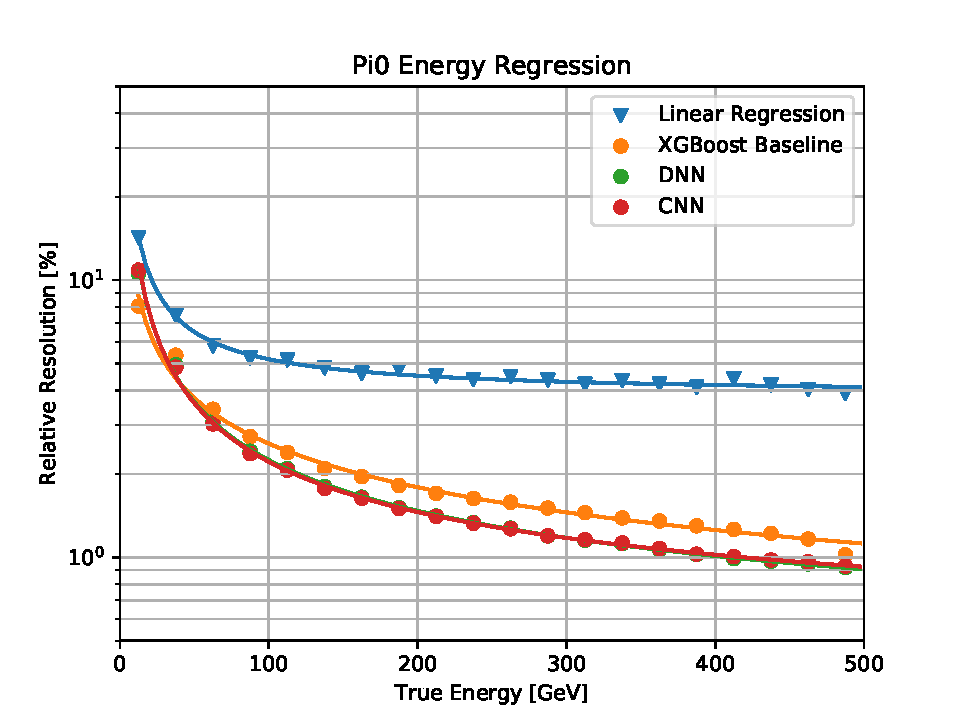
\includegraphics[width=0.45\textwidth]{Images/Calo/res_vs_E_Pi0Fixed_nn_vs_cnn_fits.pdf}
\caption{Regression bias (left) and resolution (right) as a function of true energy for energy predictions on the REC dataset with fixed incident angle ($90^\mathrm{o}$). From top to bottom: electrons, charged pions, photons, and neutral pions.\label{fig:reg_dnn_vs_cnn_fixed}}
\end{figure*}

\subsection*{Cross Training on Different Particle Types}

All the tests so far have assumed that we know exactly what type of particle led to the reconstructed energy deposits.  In a real world situation, the particle identities are not known with complete confidence.  To see how the algorithms above would cope with that situation, we tried training each algorithm on an input sample of electron events, and then we used the trained algorithm to predict the energies for other particle types.

The results are shown in Figure~\ref{fig:reg_nn_cross_gamma} for predicting photon energies and Figure~\ref{fig:reg_nn_cross_pi0} for predicting \pizero\ energies, and are compared to algorithms that are both trained and tested on the same particle type.  In each case, a DNN or CNN trained on electrons is able to achieve the same resolution as a CNN trained on photons or \pizero.  The bias is slightly larger in some cases.

\begin{figure}[hbp]
\centering
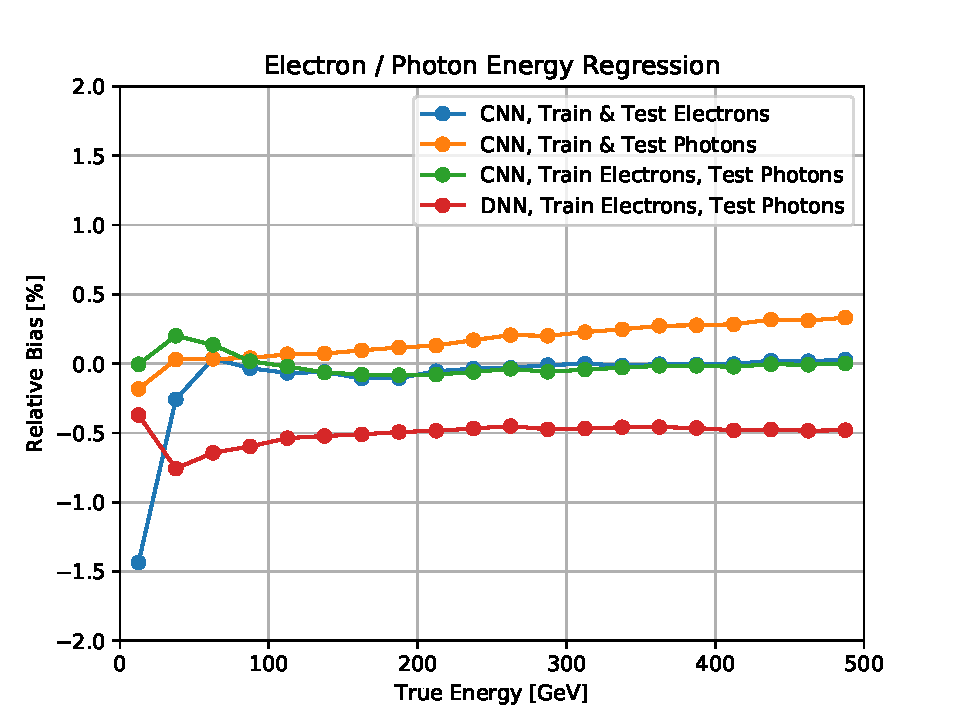
\includegraphics[width=0.45\textwidth]{Images/Calo/bias_vs_E_EleGammaFixed_nn_cross_zoom.pdf}
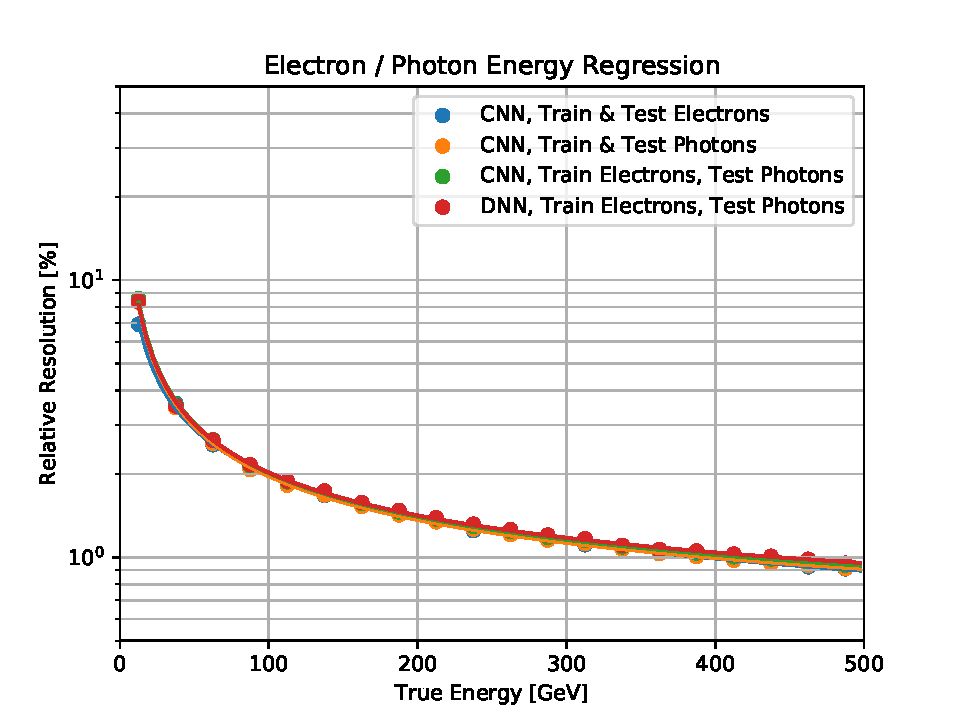
\includegraphics[width=0.45\textwidth]{Images/Calo/res_vs_E_EleGammaFixed_nn_cross_fits.pdf}
\caption{Bias (left) and resolution (right) as a function of true energy, for electrons and photons.  The particles used to train and test each algorithm are given in the legend.
}
\label{fig:reg_nn_cross_gamma}
\end{figure}

\begin{figure}[htbp]
\centering
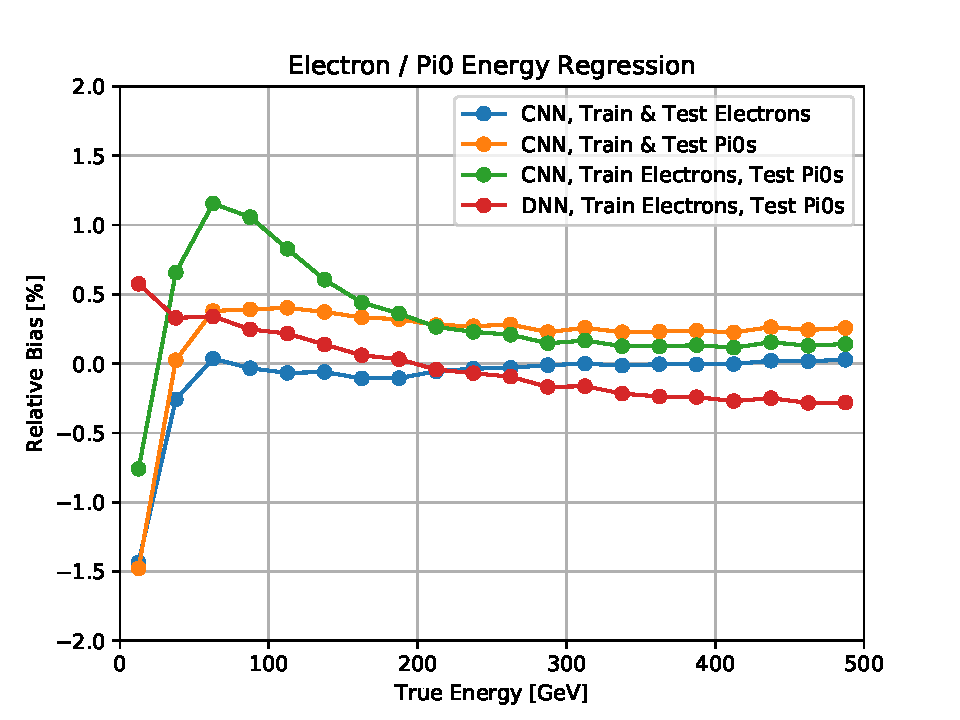
\includegraphics[width=0.45\textwidth]{Images/Calo/bias_vs_E_ElePi0Fixed_nn_cross_zoom.pdf}
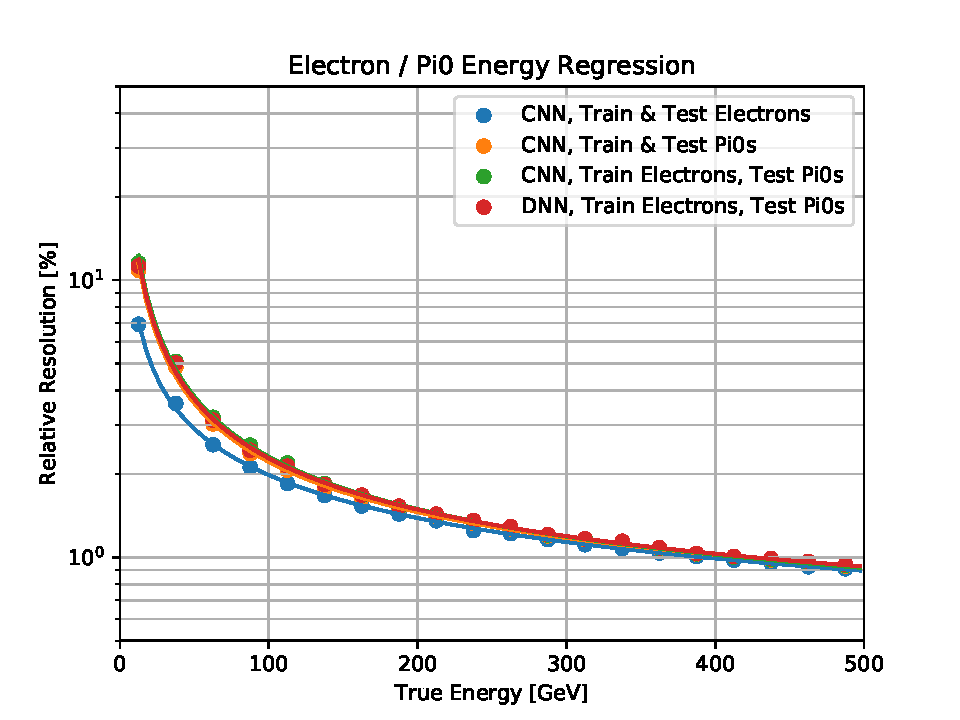
\includegraphics[width=0.45\textwidth]{Images/Calo/res_vs_E_ElePi0Fixed_nn_cross_fits.pdf}
\caption{Bias (left) and resolution (right) as a function of true energy, for electrons and \pizero.  The particles used to train and test each algorithm are given in the legend.
}
\label{fig:reg_nn_cross_pi0}
\end{figure}

Models trained on electrons, photons, or \pizero\ were found to not describe \chpi\ well at all.  This is not surprising given that \chpi\ has a hadronic shower, with a large fraction of energy deposited in the HCAL, compared to the other particles depositing almost all of their energy in the ECAL.

We also checked whether the energy regression was different for photons that have converted into an $e^{+}e^{-}$ pair through interaction with the detector material.  These conversion photons comprise about 9\% of the photon sample.  We tried training and/or evaluating regression models separately on converted photons compared to all photons (which are dominated by unconverted).  The results are shown for XGBoost in Figure~\ref{fig:reg_xgb_conv_gamma} and for CNN/DNN models in Figure~\ref{fig:reg_nn_conv_gamma}.  Worse resolution is seen in each case for converted photons below around 100~GeV, which can be attributed to the subsequent electrons forming two showers instead of one in the calorimeter.  With XGBoost, the resolution remains the same for converted photons when training on the full sample, while for CNN or DNN, the resolution is worse below around 100~GeV.  The bias is also worse for converted photons at lower energy when training on all photons.

\begin{figure}[htbp]
\centering
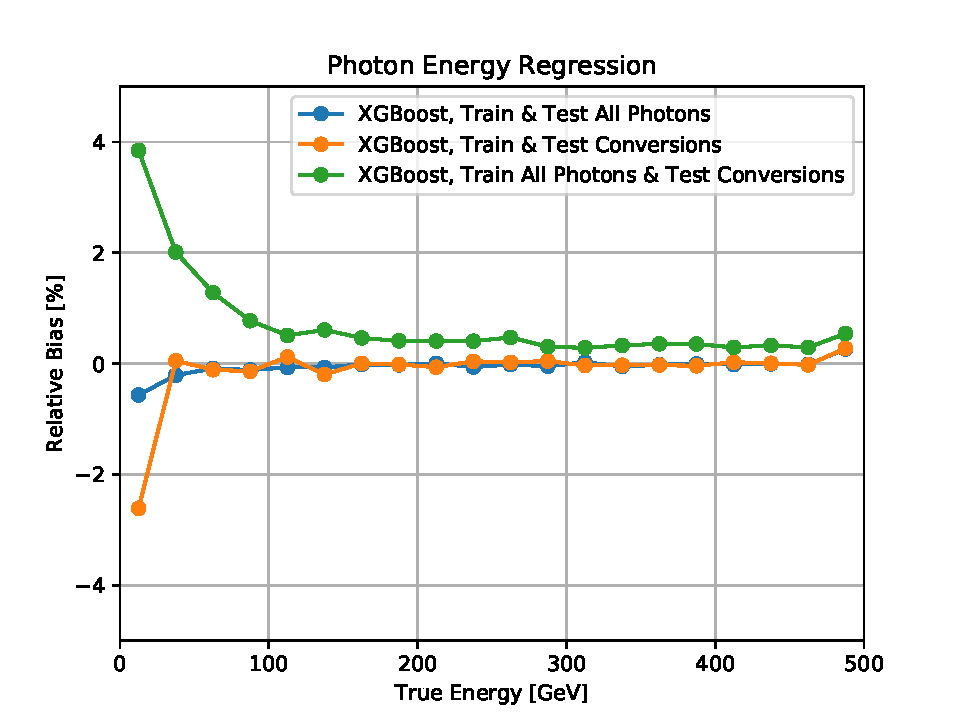
\includegraphics[width=0.45\textwidth]{Images/Calo/bias_vs_E_GammaFixed_xgb_convs.pdf}
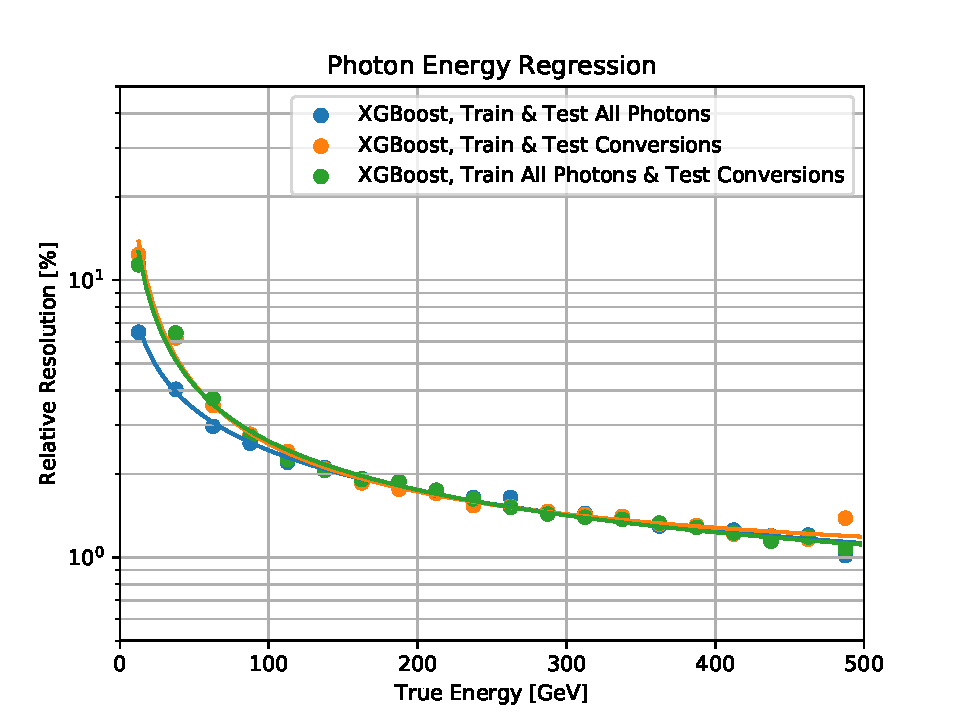
\includegraphics[width=0.45\textwidth]{Images/Calo/res_vs_E_GammaFixed_xgb_convs_fits.pdf}
\caption{Bias (left) and resolution (right) as a function of true energy, for photons using XGBoost regression.  We look at the photon sample when split up by conversions.
}
\label{fig:reg_xgb_conv_gamma}
\end{figure}

\begin{figure}[htbp]
\centering
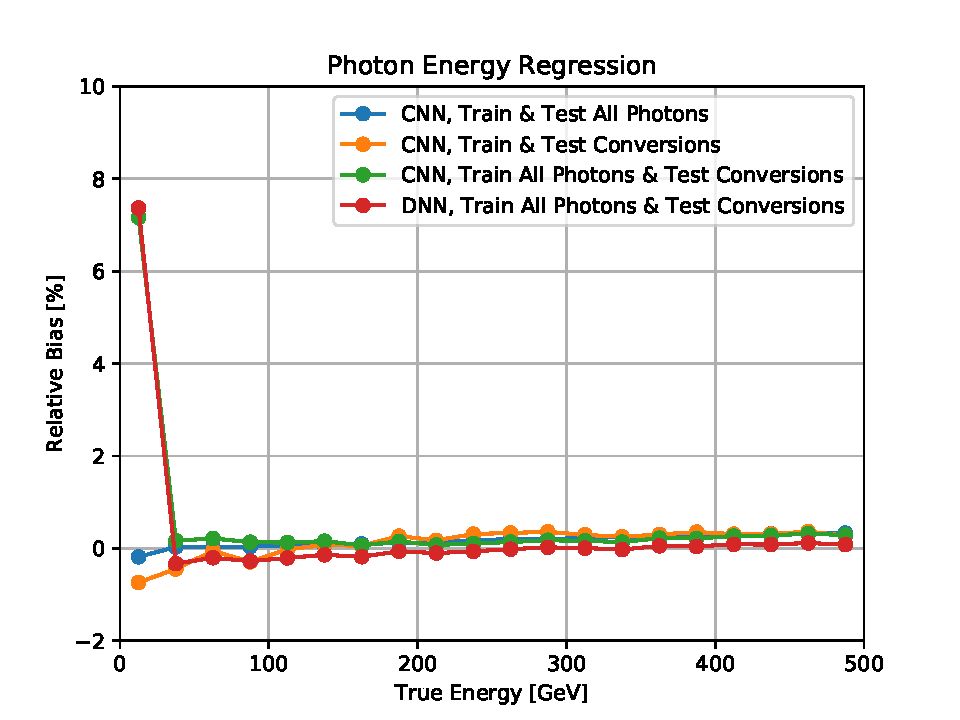
\includegraphics[width=0.45\textwidth]{Images/Calo/bias_vs_E_GammaFixed_nn_convs.pdf}
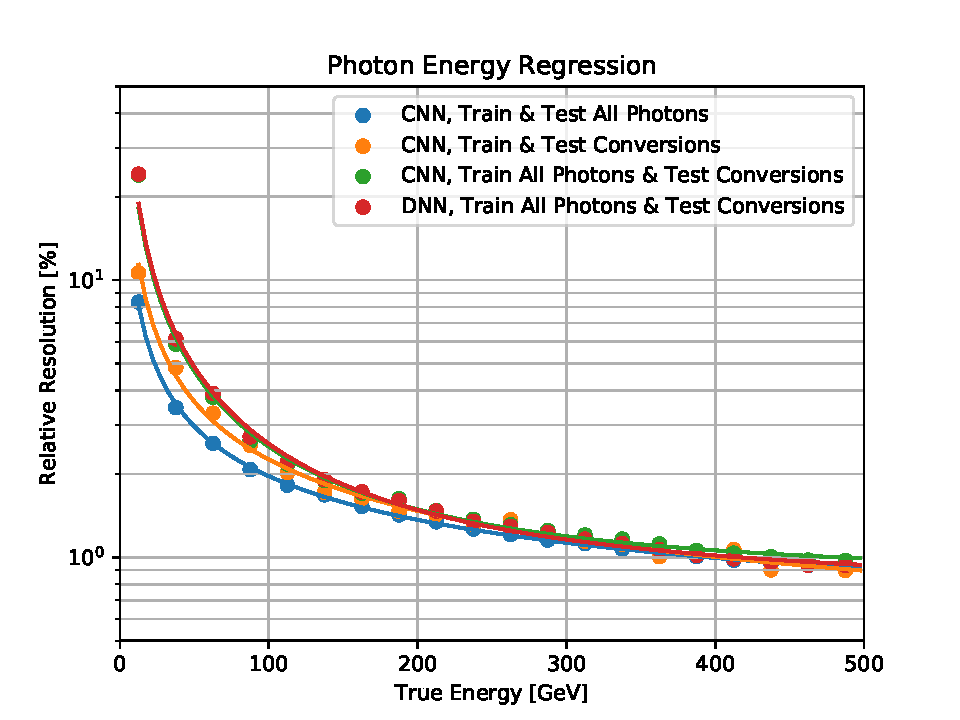
\includegraphics[width=0.45\textwidth]{Images/Calo/res_vs_E_GammaFixed_nn_convs_fits.pdf}
\caption{Bias (left) and resolution (right) as a function of true energy, for photons using CNN or DNN regression.  We look at the photon sample when split up by conversions.
}
\label{fig:reg_nn_conv_gamma}
\end{figure}

\section{Resampling to ATLAS and CMS Geometries}\label{sec:resampling}

In addition to the results presented so far, we show in this section how the end-to-end reconstruction would perform on calorimeters with granularity and geometry similar to those of the ATLAS and CMS calorimeters. Since the REC dataset (see Section~\ref{sec:data}) is generated using the geometry of the proposed LCD detector, it has a much higher granularity than the current-generation ATLAS and CMS detectors. To visualize how our calorimeter data would look with a coarser detector, we linearly extrapolate the contents of each event to a different calorimeter geometry, using a process we have termed "resampling". To keep the resampling procedure simple, we discard the HCAL information and consider only the ECAL 3D array.

A not-to-scale example of the full procedure is shown in Figure~\ref{fig:resampling}. In this example, we resample the input to a regular square grid with lower granularity than the input data. The operation is simplified in the figure, in order to make the explanation easy to visualize. The actual ATLAS and CMS calorimeter geometries are more complex than a regular array, as described in Table~\ref{tab:resampling_geometry}.

\begin{figure}[htbp]
    \centering
    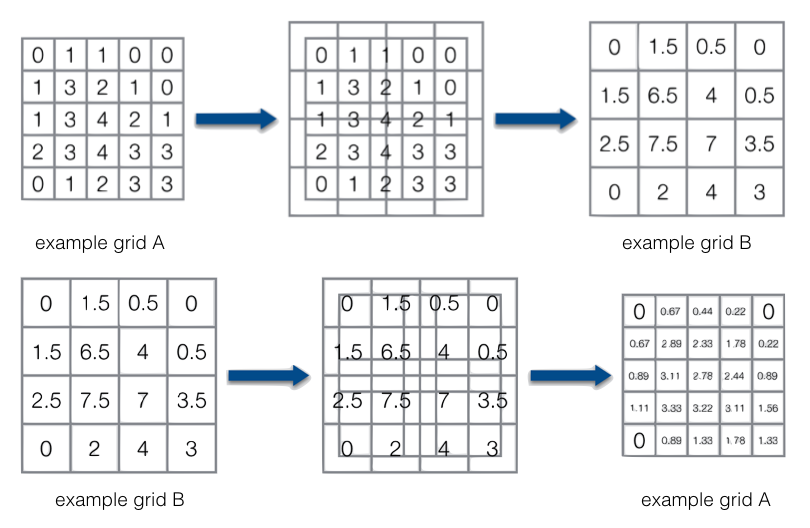
\includegraphics[scale=0.3, clip]{Images/Calo/resampling.png}
    \caption{Example of the resampling procedure used to emulate CLIC data on a different detector geometry (the example shown here is simply a larger grid). First, we extrapolate hit information from one geometry to another (top). Next, we extrapolate back to the original geometry (bottom). This allows us to emulate the rougher granularity of the second geometry, while keeping data array sizes constant and enabling us to use the models we have already developed for the CLIC dataset. Note that some information is lost at the edges.}
    \label{fig:resampling}
\end{figure}

\begin{table*}[htbp]
\centering
\caption{Detailed description of the three detector geometries used in this study: the baseline CLIC ECAL~\cite{CLIC_geometry} and the ATLAS~\cite{Aad:2008zzm} and CMS~\cite{Chatrchyan:2008aa} ECALs.\label{tab:resampling_geometry}}
\begin{tabular}{c|c|ccc|c}
\hline
\multirow{2}{*}{Parameter} & \multirow{2}{*}{\textbf{CLIC}} & \multicolumn{3}{c|}{\textbf{ATLAS}} & \multirow{2}{*}{\textbf{CMS}} \\
            &               & 1st layer & 2nd layer & 3rd layer & \\
\hline
$\Delta \eta$         & 0.003  & 0.025 /8 & 0.025 & 0.5   & 0.0175 \\
$\Delta \phi$         & 0.003  & 0.1      & 0.025 & 0.025 & 0.0175 \\
Radiation Length [cm] & 0.3504 & 14       & 14    & 14    & 0.8903 \\
Moliere radios [cm]   & 0.9327 & 9.043    & 9.043 & 9.043 & 1.959  \\
\hline 
\end{tabular}
\end{table*}

In the resampling process, we first extrapolate each energy value from the grid of CLIC cells to a different geometry. To do so, we scale the content of each CLIC cell to the fraction of overlap area between the CLIC cell and the cell of the target geometry. When computing the overlap fraction, we take into account the fact that different materials have different properties (Moliere radius, interaction length, and radiation length). For instance, CLIC is more fine-grained than CMS or ATLAS detectors, but the Moliere radius of the CLIC ECAL is much smaller than in either of those detectors. This difference determines an offset in the fine binning. Thus, when applying our resampling procedure we normalize the cell size by the detector properties. The Moliere radius is used for $x$ and $y$ re-binning, and radiation length is used for the $z$ direction. At this point we have a good approximation for how the event would look in a calorimeter with the target geometry.

To complete the resampling process, we invert the procedure to go back to our original high-granularity geometry. This last step allows us to keep using the model architectures that we have already optimized. It adds no additional information that would not be present in the low-granularity geometry. This up-sampling also allows us to deal with the irregular geometry of the ATLAS calorimeter by turning it into a neat grid. With no up-sampling, it would not be possible to apply the CNN and GN models. This procedure was validated by comparing total energies before and after resampling, and by visually comparing resampled grids. The energy matches for events were not exact, due to losses at the edge of the resampling grid, and the shower resolutions became much less granular after resampling, but overall the energies and distributions matched before and after the procedure was applied.

%\begin{center}
%\begin{tabular}{ l | c c c c c }
% Detector & Cell Size ($\Delta\eta\times\Delta\phi$) & Image Size & Material & $\Chi_0$ [cm] & $R_M$ [cm] \\ 
%\hline
%CLIC          & $0.003\times0.003$     & $25\times25\times25$ & tungsten & 0.35 & 0.92       \\
%CMS           & $0.0175\times0.0175$   & $5\times5\times1$    & lead tungstate & 0.89 & 1.96 \\  
%ATLAS layer 1 & $0.003\times0.1$       & & & & \\
%\caption{Calorimeter properties for the three detector geometries considered. UPDATE FORMAT TO FIT IN ONE COLUMN AND ADD ATLAS 3 LAYERS}
%\end{tabular}
%\end{center}

The resampling procedure comes with a substantial simplification of the underlying physics process. First of all, the information at the edge of the grid is imperfectly translated during the resampling process, leading to worse performance than what could theoretically be achieved in the actual CMS and ATLAS detectors. Also, this simple geometrical rescaling doesn't capture many other detector characteristics. For example, the CMS ECAL detector has no depth information, but being homogeneous it provides a very precise energy measurement. Our resampling method only captures geometric effects, and would not be able to model the improvement in energy resolution. Furthermore, we are unable to include second-order effects such as gaps in the detector geometries. Despite these limitations, one can still extract useful information from the resampled datasets, comparing the classification and regression performances of our neural architectures on different detector geometries.

Comparisons of classification ROC curves between network architectures and our BDT baseline are shown in Figure~\ref{fig:class_ROC_ATLAS_CMS} for ATLAS-like and CMS-like geometries. Here we can see that the previously observed performance ranking still holds true. The GN
model performs best, followed by the CNN, then the DNN. All three networks outperform the BDT baseline. The effect is less pronounced after the CMS-like resampling, due to the low granularity and the single detector layer in the z direction.

\begin{figure}[htbp]
    \centering
    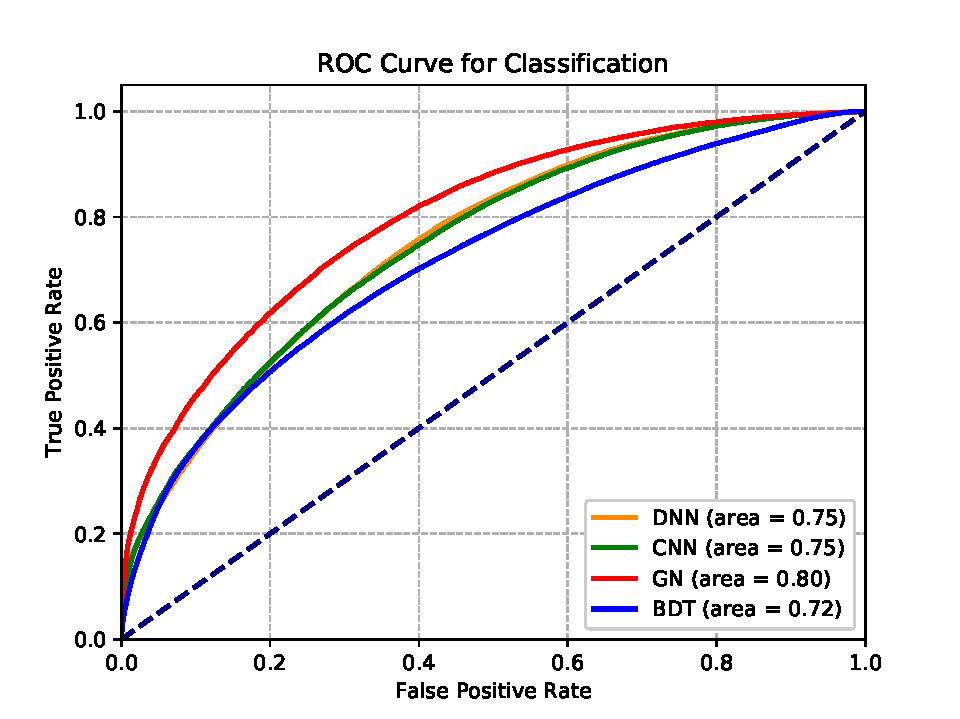
\includegraphics[width=0.45\textwidth]{Images/Calo/classification_ROC_ATLAS.pdf}
    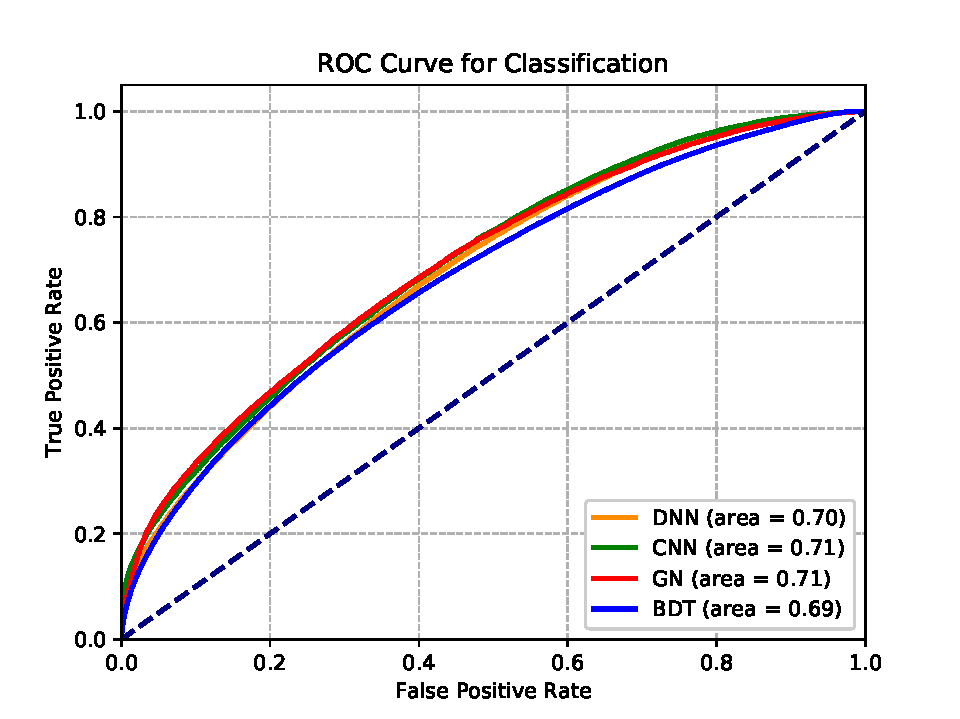
\includegraphics[width=0.45\textwidth]{Images/Calo/classification_ROC_CMS.pdf}
    \caption{ROC curve comparisons for variable-angle $\gamma$/$\pi^0$ classification on data resampled to ATLAS-like (left) and CMS-like (right) geometries. Algorithms compared are DNN, CNN, GoogLeNet (GN), and BDT.}
    \label{fig:class_ROC_ATLAS_CMS}
\end{figure}

Regression results are shown in Figure~\ref{fig:reg_resampled_gamma_ATLAS_CMS} and~\ref{fig:reg_resampled_pi0_ATLAS_CMS}, for photons and neutral pions (we did not train electrons or charged pions for this comparison). Here we have included the regression baselines, DNN networks, and CNN networks, but not GN (which we did not train on resampled data). The results obtained for the ATLAS-like resampling match those on the REC dataset, with DNN and CNN matching the BDT outcome in terms of bias and surpassing it in resolution. With the CMS-like resampling the neural networks match but do not improves over the BDT energy regression resolution. Once again, this is due to the low spatial resolution in the CMS-like geometry, especially due to the lack of $z$ segmentation. We are unable to model the improved energy resolution from the actual CMS detector, so these energy regression results are based on geometry only.

\begin{figure*}[htbp]
\centering
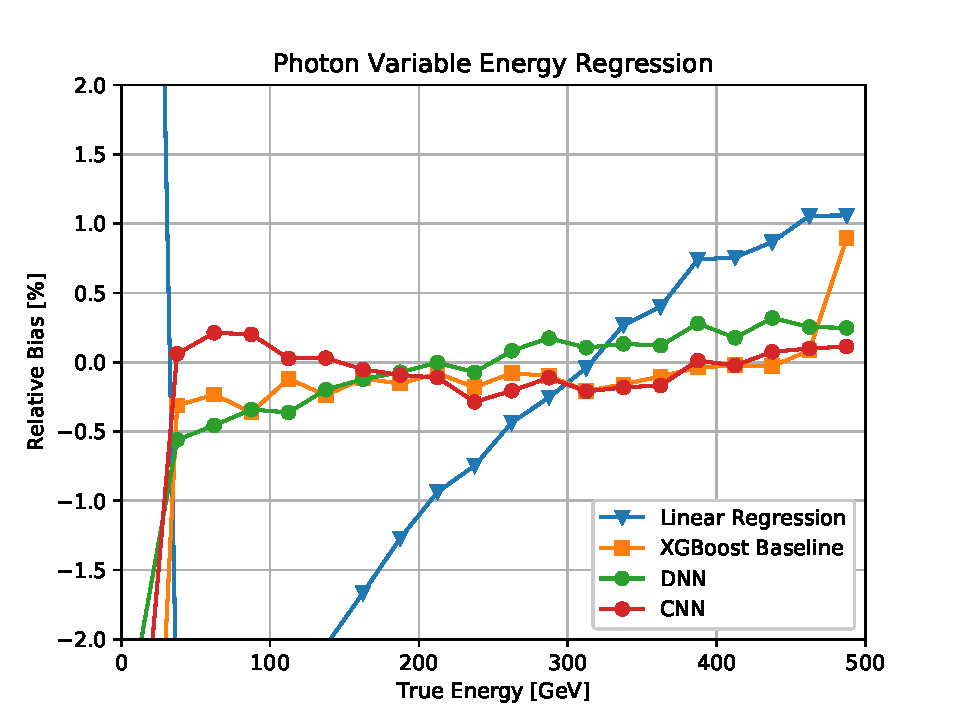
\includegraphics[width=0.45\textwidth]{Images/Calo/bias_vs_E_Gamma_variable_ATLAS.pdf}
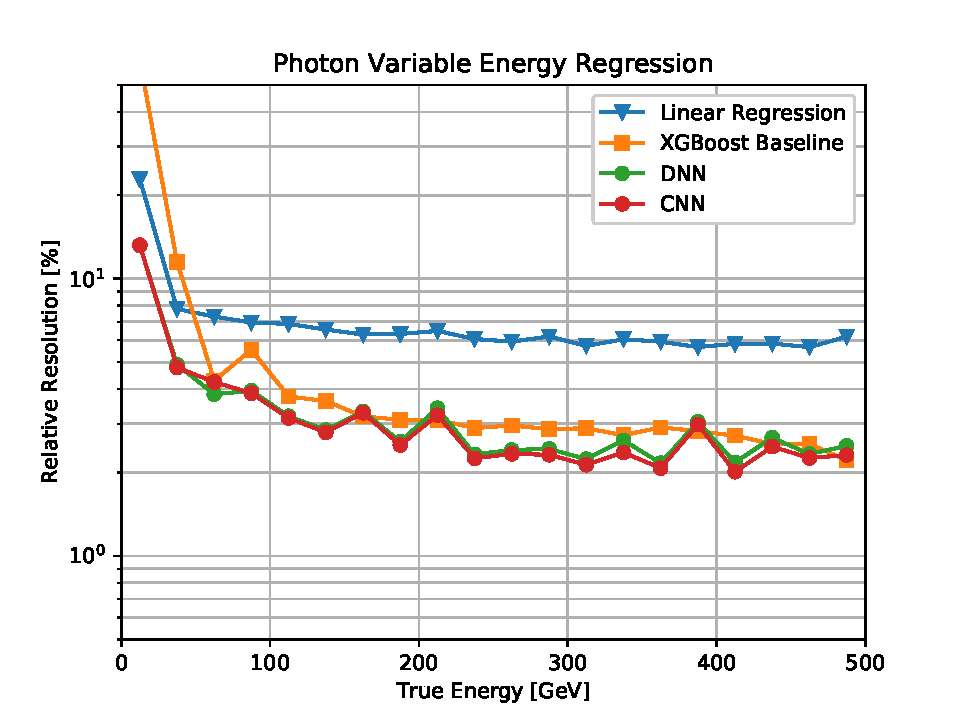
\includegraphics[width=0.45\textwidth]{Images/Calo/res_vs_E_Gamma_variable_ATLAS.pdf} \\
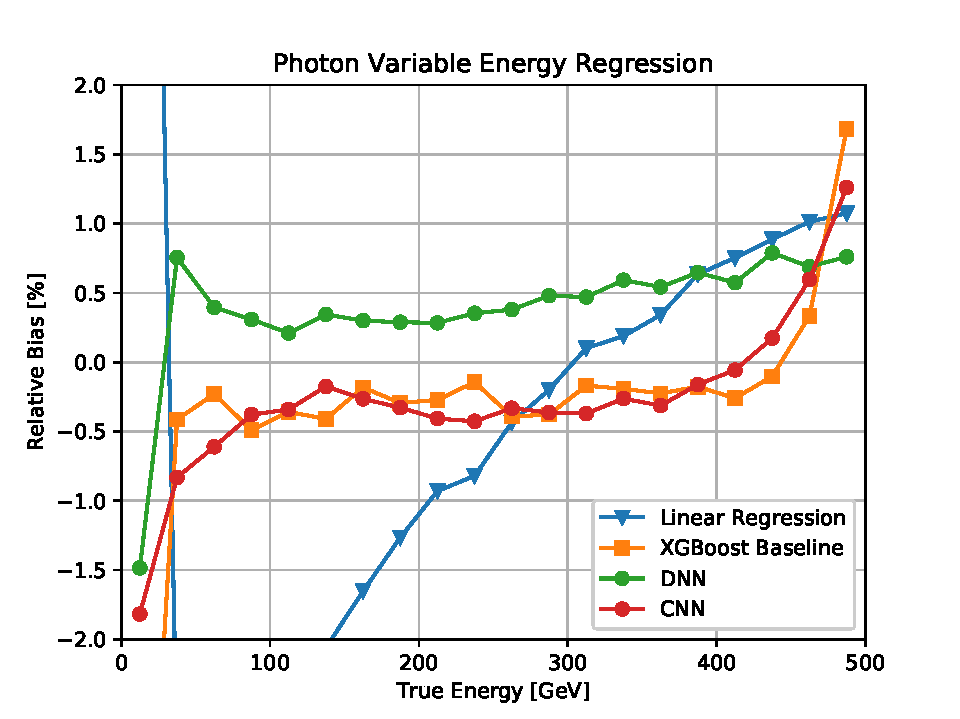
\includegraphics[width=0.45\textwidth]{Images/Calo/bias_vs_E_Gamma_variable_CMS.pdf}
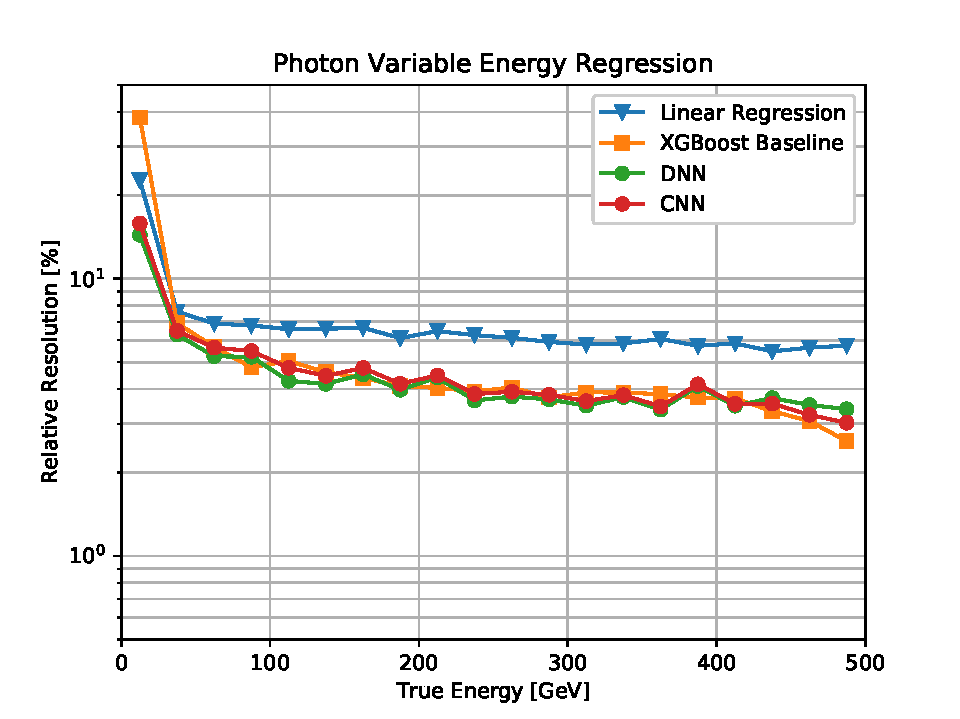
\includegraphics[width=0.45\textwidth]{Images/Calo/res_vs_E_Gamma_variable_CMS.pdf}
\caption{Bias (left) and resolution (right) as a function of true energy for energy predictions for photons, on variable-angle samples resampled to ATLAS-like (top) and CMS-like (bottom) geometries. \label{fig:reg_resampled_gamma_ATLAS_CMS}}
\end{figure*}

\begin{figure*}[htbp]
\centering
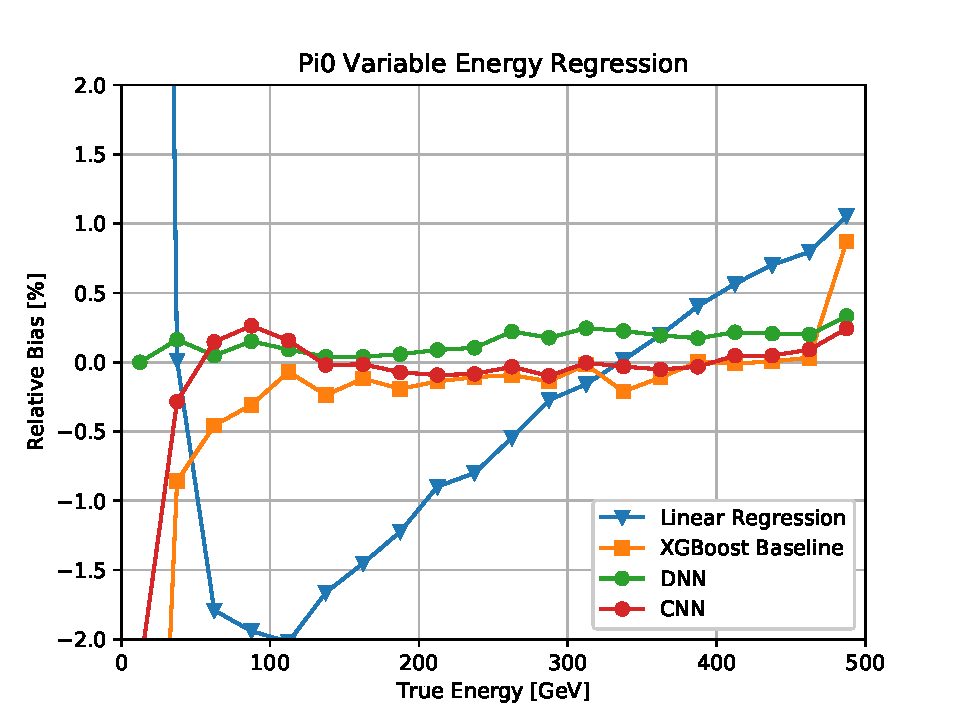
\includegraphics[width=0.45\textwidth]{Images/Calo/bias_vs_E_Pi0_variable_ATLAS.pdf}
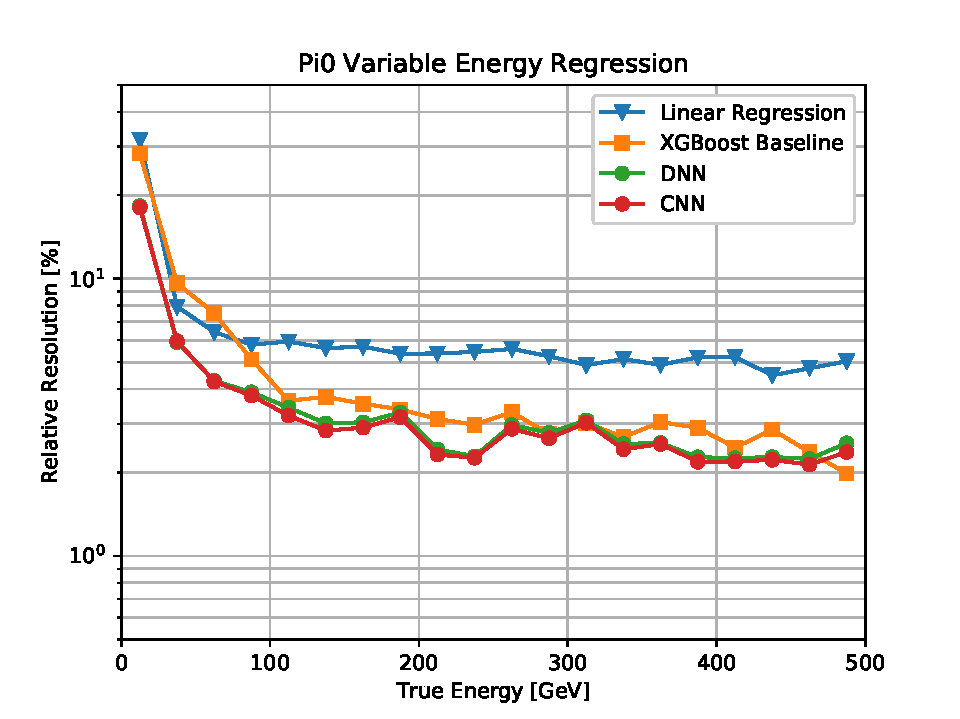
\includegraphics[width=0.45\textwidth]{Images/Calo/res_vs_E_Pi0_variable_ATLAS.pdf} \\
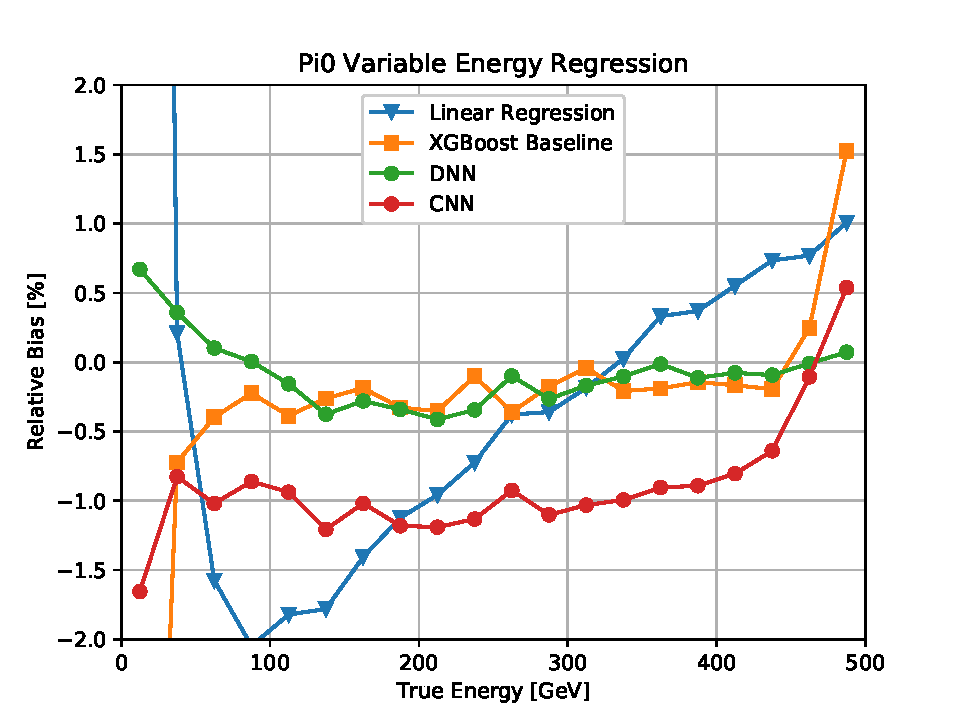
\includegraphics[width=0.45\textwidth]{Images/Calo/bias_vs_E_Pi0_variable_CMS.pdf}
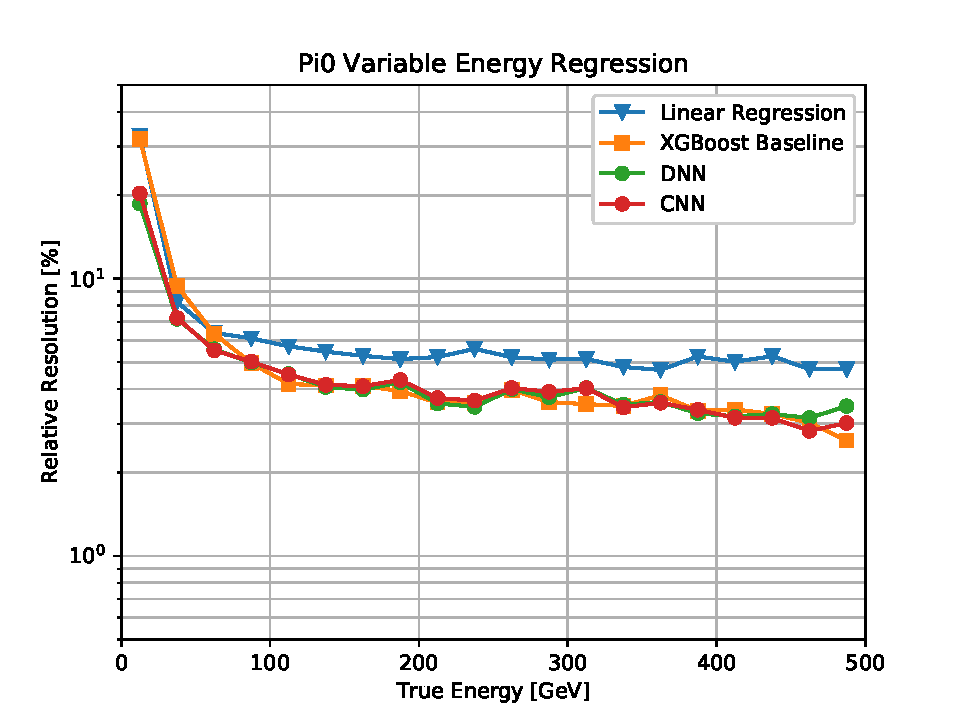
\includegraphics[width=0.45\textwidth]{Images/Calo/res_vs_E_Pi0_variable_CMS.pdf}
\caption{Bias (left) and resolution (right) as a function of true energy for energy predictions for \pizero, on variable-angle samples resampled to  ATLAS-like (top) and CMS-like (bottom) geometries.\label{fig:reg_resampled_pi0_ATLAS_CMS}}
\end{figure*}